\documentclass[10pt, twoside, a4paper]{article}
\usepackage{fancyhdr}
\usepackage{amsmath, amsthm, amssymb}
\usepackage[catalan]{babel}
\usepackage[titles]{tocloft}
\usepackage[utf8]{inputenc}
\usepackage[left=2.15cm, right=2.15cm, top=30mm, bottom=20mm]{geometry}
\usepackage{parskip}
\usepackage{subcaption}
\usepackage{titlesec}
\usepackage{bookmark}
\usepackage{multirow}
\usepackage{graphicx}
\usepackage{physics}
\usepackage{hyperref}
\usepackage{float}
\usepackage{caption}
\captionsetup{labelfont=bf}
\begin{document}

\begin{titlepage}
\centering
{\LARGE Mètodes Numèrics II \par}
\vspace{2cm}
{\Huge \textbf{Pràctica de simulació:} \par}
\vspace{1cm}
{\Huge \textbf{TITOLTITOLTITOL} \par}
\vspace{3cm}
{\Large G01 \par}
\vspace{0.5cm}
{\Large 1548086: Bujones Umbert, Jun Shan\\1666739: Franco Avilés, Eric\\  1672980: González Barea, Eric\\1644841: Vilarrúbias Morral, Natàlia \par}
\vspace{2cm}
{\Large Gener 2025 \par}
\vspace{2cm}

\includegraphics[width=0.4\textwidth]{Logo_UAB.png}


\end{titlepage}

\pagenumbering{gobble}
\renewcommand{\cftsecfont}{}
\renewcommand{\cftsecpagefont}{}
\renewcommand{\cftsecleader}{\cftdotfill{\cftdotsep}}
\renewcommand{\cftdotsep}{0.2}
\setlength{\cftbeforesecskip}{0.5em}
\setlength{\cftbeforesubsecskip}{0.5em}
\tableofcontents

\newpage
\pagenumbering{arabic}
\setcounter{page}{1}

\pagestyle{fancy}
\lhead{\textbf{Pràctica de Simulació}}
\rhead{\textbf{Mètodes Numèrics II}}

\section{Introducció}
Here goes \textit{blahblahblah}

\section{Plantejament del problema del Sistema Solar}

\subsection{Modelització del Sistema Solar}
Per tal de modelitzar el Sistema Solar, partirem de la Segona Llei de Newton i la igualarem a la Lley de la Gravitació Universal, tot dividint per la massa del cos $p$, $M_p$. Fent això ens queda que l'acceleració a la qual està sotmesa aquest cos és:

\begin{equation}
    \derivative[2]{\mathbf{r}^{(p)}}{t} = - G \left[ \sum_{l \neq p} M_l \frac{(\mathbf{r}^{(p)}-\mathbf{r}^{(l)})}{\abs{\mathbf{r}^{(p)} - \mathbf{r}^{(l)}}^3}\right], \hspace{0.25cm} p = 1, 2, \ldots 
\end{equation}

En aquesta equació el vector $\mathbf{r}^{(p)}$ és el vector posició (marquem els vectors en negreta) del cos $p$ respecte del Sol (de manera que el nostre origen de coordenades serà la posició inicial del Sol), $M_l$ la massa dels cossos diferents a $p$ i $\mathbf{r}^{(l)}$ les seves posicions respecte l'origen. Fixem-nos, doncs, que segons aquesta equació, la força que actua sobre un planeta donat es correspon amb la suma de les forces exercides per tots els cossos del sistema solar sobre ell. 

Simplificarem l'expressió definint $\mathbf{d}_{pl} \equiv (\mathbf{r}^{(p)}-\mathbf{r}^{(l)})$. Així, la darrera equació queda com
\begin{equation}
    \derivative[2]{\mathbf{r}^{(p)}}{t} = - G \left[ \sum_{l \neq p} M_l \frac{\mathbf{d}_{lp}}{\abs{\mathbf{d}_{lp}}^3}\right], \hspace{0.25cm} p = 1, 2, \ldots 
\end{equation}

Per tal de facilitar-ne la ressolució, podem transformar aquesta equació diferencial de segon ordre a la següent

\begin{equation}
    \derivative{\mathbf{v}^{(p)}}{t} = -G \left[ \sum_{l \neq p} M_l\frac{\mathbf{d}_{lp}}{\abs{\mathbf{d}_{lp}}^3}\right], \hspace{0.25cm} p = 1,2 \ldots \label{2}
\end{equation}

De forma que tenim ara un conjunt de $n \cross p$ (on $n$ són les dimensions) equacions diferencials de primer ordre a resoldre. A la pràctica, com que tots els planetes del sistema solar tenen orbites coplanàries (a excepció de Plutó, que no el considerarem), podem assumir que estem davant d'un problema bidimensional, de manera que tindre $2 \cross p$ EDOs de primer ordre a resoldre.

Considerarem un model en què els únics cossos del Sistema Solar són Mercuri, Venus, la Terra, Mart i Júpiter (i, naturalment, el Sol), per tal de simplificar les gràfiques. A més a més, el moviment d'aquests cossos serà al pla de l'eclíptica; no considerarem moviments en l'eix $z$. Es podrà trobar una versió més complexa (amb la modelització de tots els planetes i les corresponents gràfiques per diferents temps finals) al repositori de \textit{GitHub} (veure \ref{an:a}). 

\subsection{Normalització de les equacions}
Per tal de resoldre el problema minimitzant errors i temps de càlcul cal normalitzar \eqref{2}. Definim unes quantitats característiques del sistema: escollim $M_0 = M_s$ (la massa del Sol) i $d_0 = UA$ (unitat astronòmica), ja que així podrem treballar amb valors propers a la unitat. D'aquí se'n deriva que
\begin{equation*}
    t_0 = \sqrt{\frac{d_0^3}{M_s \cdot G}}
\end{equation*}
Usant tot això, podem arribar fàcilment a 
\begin{equation}
    \derivative[2]{\mathbf{\tilde{r}}^{(p)}}{\tilde{t}} = - \sum_{l \neq p} \frac{\mathbf{d}_{lp}}{\abs{\mathbf{d}_{lp}}^3}, \hspace{0.25cm} p = 1,2 \ldots
\end{equation}
d'on tenim que
\begin{equation}
    \boxed{\derivative{\tilde{v}_i^{(p)}}{\tilde{t}} = - \sum_{l \neq p} M_l \frac{d_{lp,i}}{\abs{\mathbf{d}_{lp}}^3} \hspace{0.25cm} p = 1,2 \ldots, \hspace{0.25cm} i = 1, 2} \label{eq5}
\end{equation}

\subsection{Condicions inicials}
Per tal de conèixer les condicions inicials de cadascun dels cossos del sistema solar modelitzat (això és, $\mathbf{r}^{(p)}$ i $\mathbf{v}^{(p)}$) hem usat la base de dades del \textit{Horizons Ephemeris Service} de la NASA, que podeu trobar a \url{https://ssd.jpl.nasa.gov/horizons/}. Agafem com a punt inicial les posicions i les velocitats el dia 01-01-2025 de tots els cossos rellevants del sistema solar.

\subsection{Mètode numèric i avaluació de l'error}
El mètode numèric utilitzat ha estat el mètode d'Euler (per sistemes EDOs)\footnote{Les corresponents equacions es poden consultar als apunts de l'assignatura.} aplicat a l'equació \eqref{eq5} per diferents discretitzacions temporals: $dt = 1$ any, $dt = 1$ mes i $dt = 1$ dia.

Per tal d'avaluar l'error comés estudiarem l'evolució de les dues quantitats conservades d'aquest sistema: el moment angular $\abs{\mathbf{L}} \equiv L$ i l'energia total $\varepsilon$. Idealment, a cada cas d'iteració el valor de $E$ i $L$ ha de ser el mateix que a $t_0$; les fluctuacions en aquestes quantitats ens permetran determinar l'error numèric comès segons:
\begin{align}
    E_{\varepsilon_i} = \left( \frac{\Delta \varepsilon_i}{\varepsilon_0} \right) & = \frac{\abs{\varepsilon_i - \varepsilon_0}}{\varepsilon_0} \\
    E_{L_i} = \left( \frac{\Delta L_i}{L_0} \right) & = \frac{\abs{L_i - L_0}}{L_0}
\end{align}

On els valors de $\varepsilon$ i $L$ es poden treure a partir de les equacions fonamentals de la dinàmica.

\section{Plantejament del problema de la placa solar}

\subsection{Modelització del moviment del Sol sobre Mont-rós}

\subsection{Normalització de les equacions}
SI CAL

\subsection{Condicions inicials}

\subsection{Mètode numèric i avaluació de l'error}
SI FEU ALGO D'AIXÒ

\section{Resultats i discussió}

\subsection{Sistema Solar}
Després d'implementar el mètode numèric s'han trobat les òrbites (per a cada valor de $dt$) fins a $t=1$ any (terrestre) que es poden veure a la figura \ref{fig1}. A la figura \ref{fig2}, per la seva banda, podem veure les òrbites per a $t=100$ anys per la discretització $t=1$ dia.
 
\begin{figure}[h]
    \centering
    
    \begin{subfigure}[b]{0.32\linewidth}
        \centering
        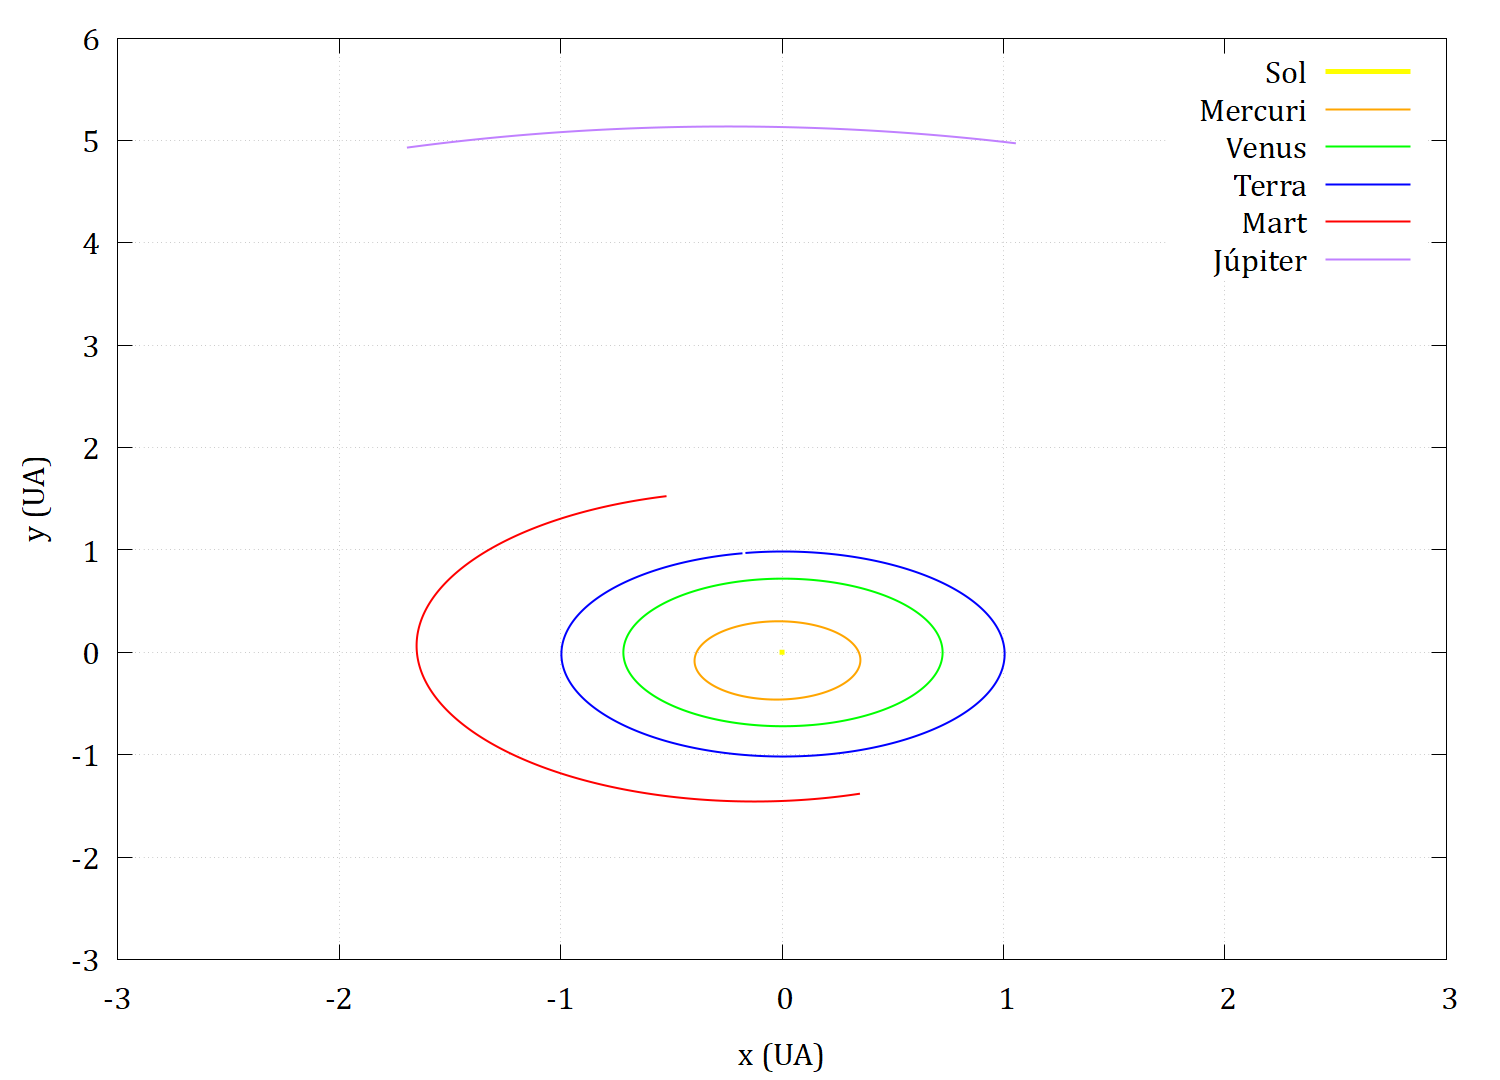
\includegraphics[width=\linewidth]{../sist_solar/orbites_euler_1_d1hora.png}
        \caption{Òrbites per $dt=1$ hora.}
        \label{fig:euler_implicit_solucio}
    \end{subfigure}
    \hfill
    \begin{subfigure}[b]{0.32\linewidth}
        \centering
        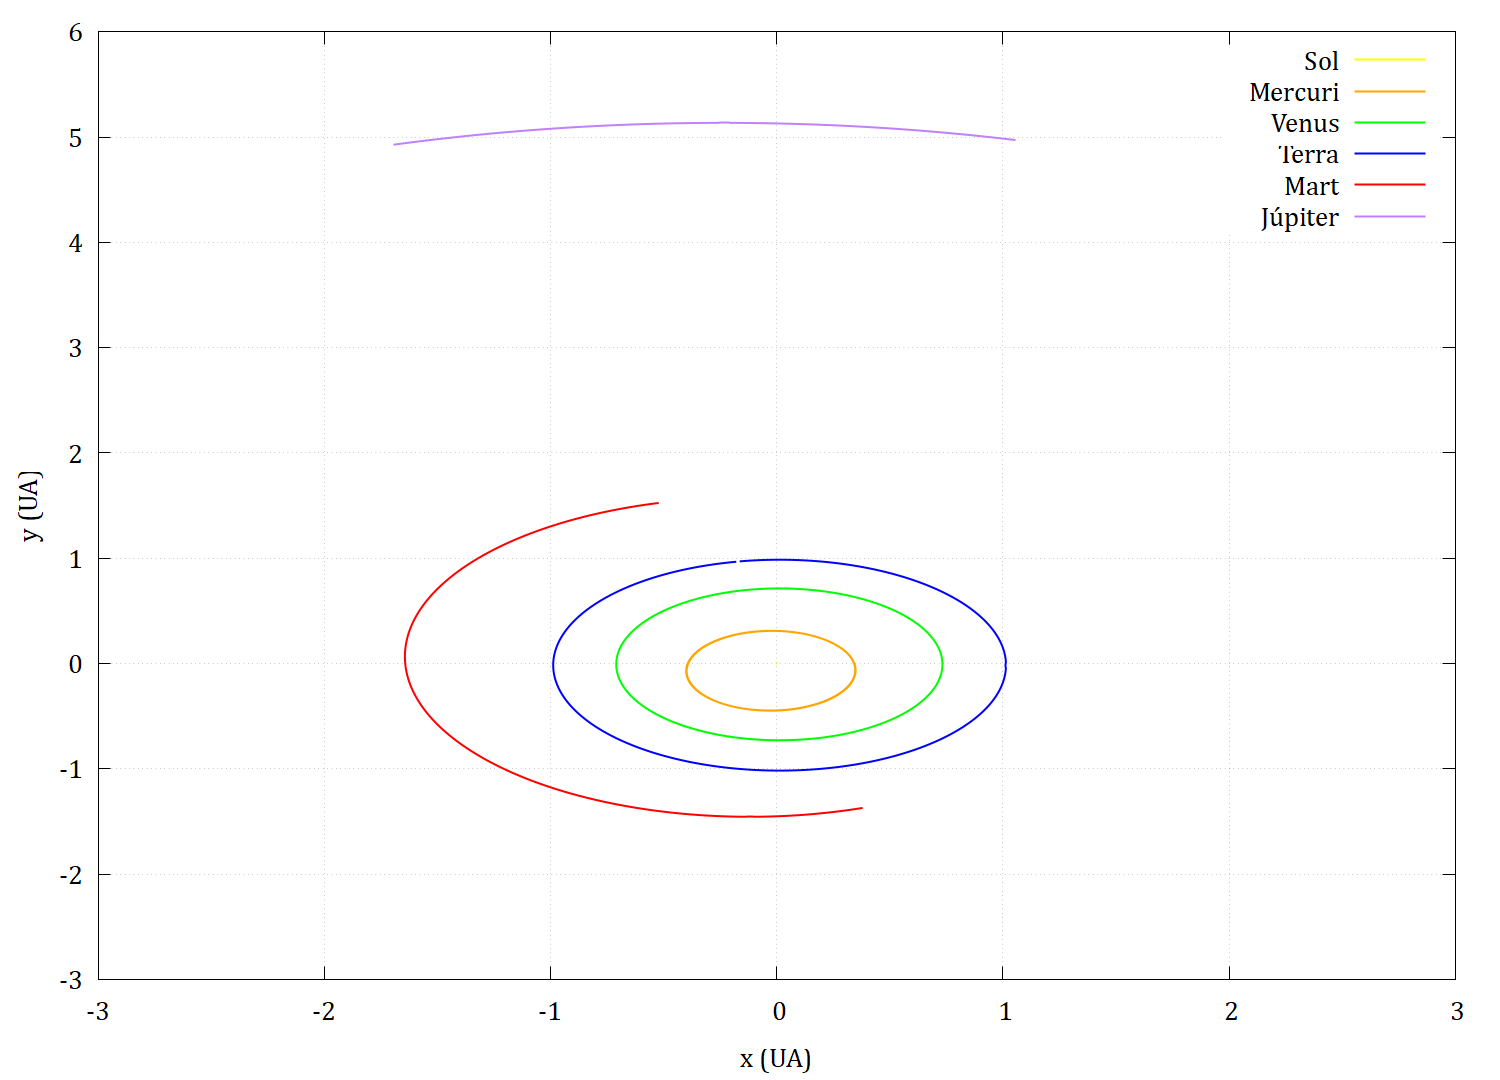
\includegraphics[width=\linewidth]{../sist_solar/orbites_euler_1_d1dia.png}
        \caption{Òrbites per $dt=1$ dia.}
        \label{fig:euler_implicit_errors}
    \end{subfigure}
    \hfill
    \begin{subfigure}[b]{0.32\linewidth}
        \centering
        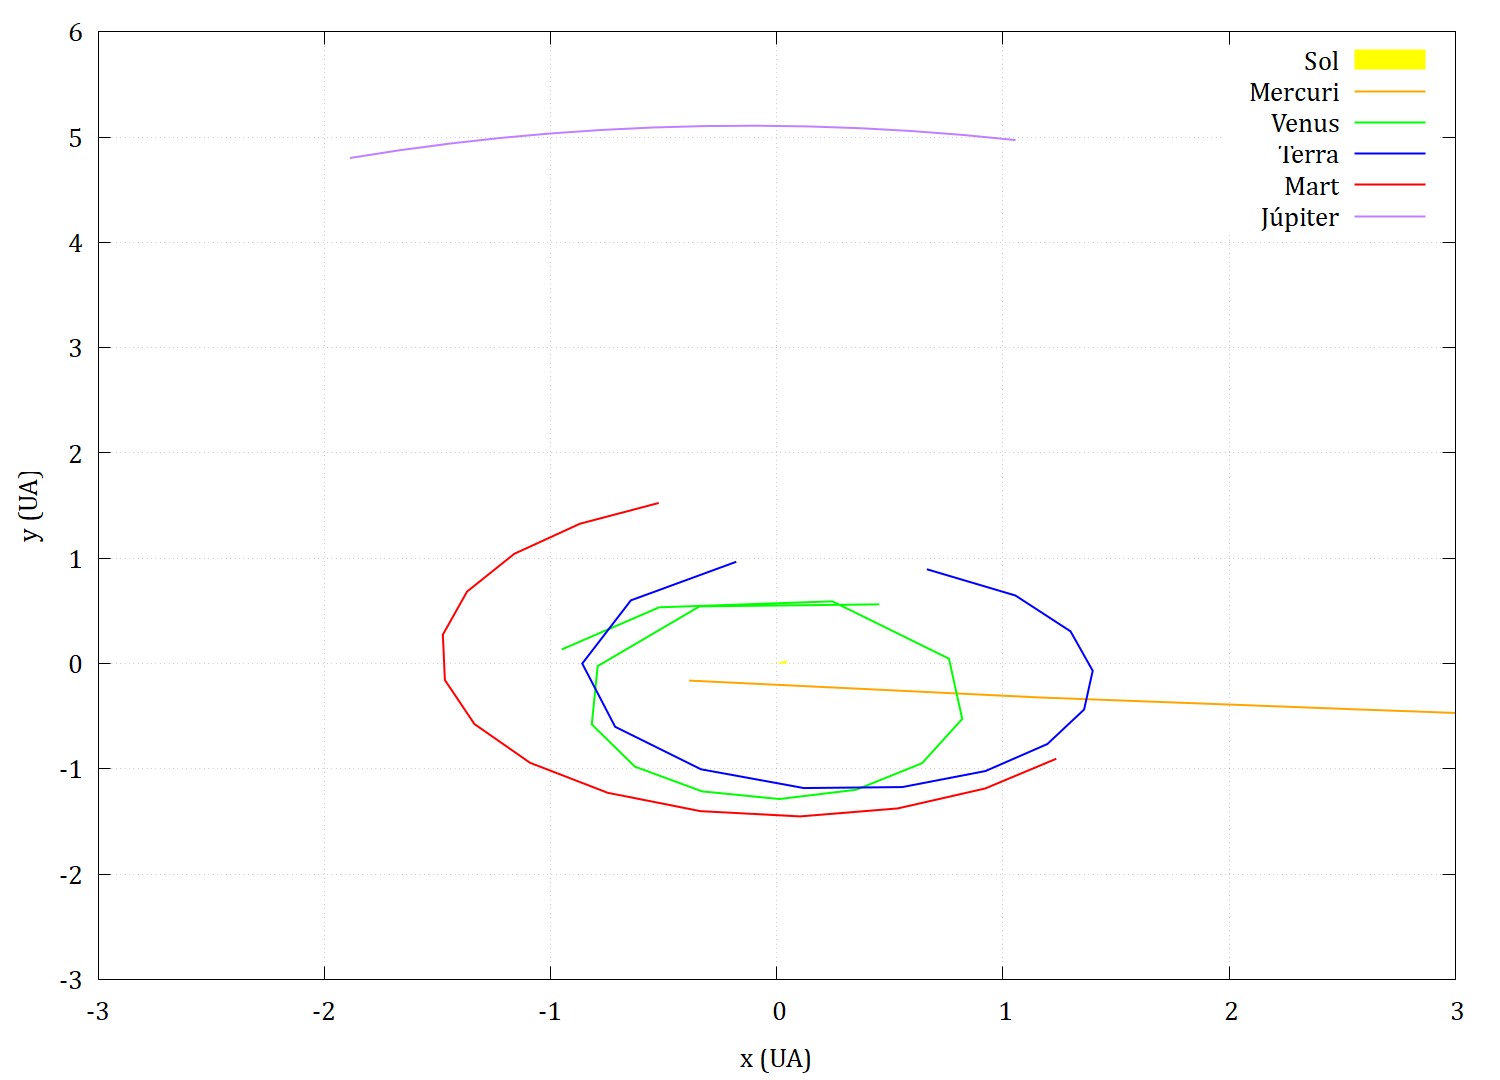
\includegraphics[width=\linewidth]{../sist_solar/orbites_euler_1_d1mes.png}
        \caption{Òrbites per $dt=1$ mes.}
        \label{fig:euler_implicit_errors}
    \end{subfigure}
    
    \caption{Òrbites del sistema solar a $t=1$ any (terrestre) per diferents valors de la discretització obtingudes.}
    \label{fig1}
\end{figure}

\begin{figure}[h]
    \centering
    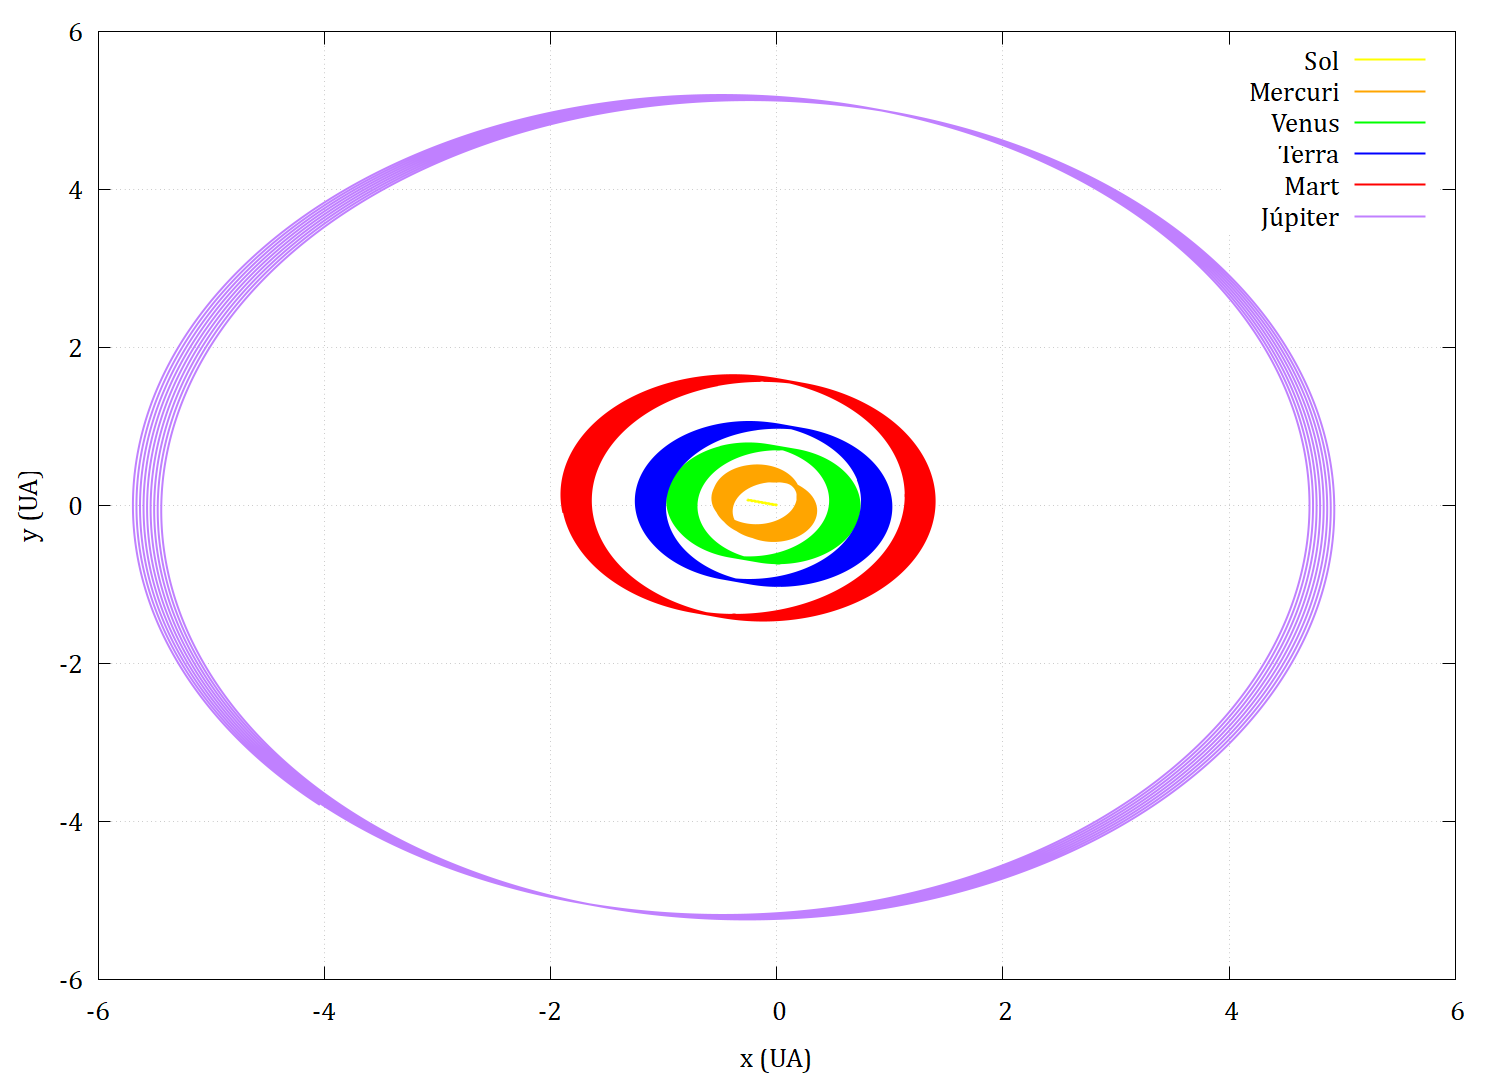
\includegraphics[width=0.5\linewidth]{../sist_solar/orbites_euler_100_1dia.png}
    \caption{Òrbites obtingudes per $t = 100$ anys amb una discretització $dt=1$ dia.}
    \label{fig2}
\end{figure}

A l'annex \ref{an:a} podeu trobar les gràfiques corresponents a tot el Sistema Solar (amb els cossos no descrits aquí) i una animació d'això últim i de les òrbites representades a la figura \ref{fig2}.

ERRORS AQUÍ!

\subsection{Moviment del Sol sobre Mont-rós}


\subsection{Energia subministrada per la placa solar}


\section{Conclusions}



\newpage
\begin{thebibliography}{99}
    \bibitem{ref1}
    \textit{Apunts de l'Assignatura}.

    \bibitem{ref2}
    Aguilar, L. \textit{Modelizando el Sistema Solar}. Consultat el: 11/12/2024. \url{https://www.astrosen.unam.mx/~aguilar/MySite/Teaching_files/BasicEqns-1.pdf}.

    \bibitem{ref3}
    \textit{Horizon Ephemeris}, NASA. Consultat el: 23/12/2024 Web de consulta de les posicions de tots els astres del sistema solar. \url{https://ssd.jpl.nasa.gov/horizons/}.

    \bibitem{ref4}
    Universidad de Granada. \textit{El Sistema Solar y las Galaxias. Una Introducción a la Dinámica Molecular}. Consultat el: 11/12/2024. \url{https://ergodic.ugr.es/cphys/LECCIONES/ssolar/planetas-SLIDES.pdf}

    
\end{thebibliography}

\newpage
\appendix
{\Huge{\textbf{Annexos}}}
\section{Repositori de \textit{GitHub}}
\label{an:a}
Podeu trobar els codis usats en \textit{Fortran}, les representacions de les gràfiques usant \textit{Gnuplot}, animacions de les simulacions del sistema solar i més al següent repositori (públic) de \textit{GitHub}: \url{https://github.com/elitus7/PSimulacio_MN2}.


\section{Normalització sistema solar}
Per tal de dur a terme la normalització definim unes quantitats característiques del sistema: $M_0 = M_s$ i $d_0 = UA$ (unitat astronòmica). Per altra banda, definim també $\mathbf{d}_{pl} = \mathbf{r}^{(p)}-\mathbf{r}^{(l)}$ (distància entre dos cossos del sistema solar).


\end{document}